\documentclass[10pt]{article}
\usepackage[UTF8]{ctex}
\usepackage{picinpar,graphicx,bm}
\usepackage{booktabs}
\usepackage{diagbox}
\usepackage{float}


\usepackage{listings}
\usepackage{xcolor}
% 定义可能使用到的颜色
\definecolor{CPPLight}  {HTML} {686868}
\definecolor{CPPSteel}  {HTML} {888888}
\definecolor{CPPDark}   {HTML} {262626}
\definecolor{CPPBlue}   {HTML} {4172A3}
\definecolor{CPPGreen}  {HTML} {487818}
\definecolor{CPPBrown}  {HTML} {A07040}
\definecolor{CPPRed}    {HTML} {AD4D3A}
\definecolor{CPPViolet} {HTML} {7040A0}
\definecolor{CPPGray}  {HTML} {B8B8B8}
\lstset{
    columns=fixed,    
   % numbers=left,                                        % 在左侧显示行号
    frame=none,                                          % 不显示背景边框
    backgroundcolor=\color[RGB]{245,245,244},            % 设定背景颜色
    keywordstyle=\color[RGB]{40,40,255},                 % 设定关键字颜色
    numberstyle=\footnotesize\color{darkgray},           % 设定行号格式
    commentstyle=\it\color[RGB]{0,96,96},                % 设置代码注释的格式
    stringstyle=\rmfamily\slshape\color[RGB]{128,0,0},   % 设置字符串格式
    showstringspaces=false,                              % 不显示字符串中的空格
    language=c++,                                        % 设置语言
    morekeywords={alignas,continute,friend,register,true,alignof,decltype,goto,
    reinterpret_cast,try,asm,defult,if,return,typedef,auto,delete,inline,short,
    typeid,bool,do,int,signed,typename,break,double,long,sizeof,union,case,
    dynamic_cast,mutable,static,unsigned,catch,else,namespace,static_assert,using,
    char,enum,new,static_cast,virtual,char16_t,char32_t,explict,noexcept,struct,
    void,export,nullptr,switch,volatile,class,extern,operator,template,wchar_t,
    const,false,private,this,while,constexpr,float,protected,thread_local,
    const_cast,for,public,throw,std,size_t,__global__,__device__,__host__},
    emph={map,set,multimap,multiset,unordered_map,unordered_set,
    unordered_multiset,unordered_multimap,vector,string,list,deque,
    array,stack,forwared_list,iostream,memory,shared_ptr,unique_ptr,
    random,bitset,ostream,istream,cout,cin,endl,move,default_random_engine,
    uniform_int_distribution,iterator,algorithm,functional,bing,numeric,},
    emphstyle=\color{CPPViolet}, 
    frame=shadowbox,
    basicstyle=\footnotesize\ttfamily,
    tabsize=4,
}


%layout
\usepackage{calc} 
\setlength\textwidth{7in} 
\setlength\textheight{9in} 
\setlength\oddsidemargin{(\paperwidth-\textwidth)/2 - 1in}
\setlength\topmargin{(\paperheight-\textheight -\headheight-\headsep-\footskip)/2 - 1.5in}


\title{计算机图形学 \hspace{2pt}\hspace{2pt} \begin{large}----- \hspace{2pt} 区域扫描线Z-Buffer算法 \end{large} }
\author{11821095 葛林林}
\begin{document}
\maketitle


\section{预备知识}
\subsection{$obj$文件}
obj文件并不考虑物体的大小,所以不同的物体读入的坐标范围可能变化很大,因此为了现实的方便需要将其转为规范化设备坐标。

\bm{顶点的表示:}顶点以$v$开头后面跟着该顶点的$x,y,z$三轴坐标,示例如下
$$format. \hspace{15pt} v\hspace{5pt} x\hspace{5pt}y\hspace{5pt}z$$
$$e.g. \hspace{15pt} v\hspace{5pt} -57.408021\hspace{5pt}196.143694\hspace{5pt}2.816352$$

\bm{纹理坐标的表示:}纹理坐标以$vt$开头。
$$format.\hspace{15pt} vt \hspace{5pt}tu \hspace{5pt} tv$$
$$$$

\bm{法向量的表示:}法向量的表示以$vn$开头。
$$format.\hspace{15pt} vn \hspace{5pt} nx \hspace{5pt} ny \hspace{5pt} nz$$
$$e.g. \hspace{15pt} vn \hspace{5pt} 5.9333 \hspace{5pt} -0.4798 \hspace{5pt} -1.8985$$

\bm{面的表示:}面以$f$开头,代表”face”的意识,格式为“f 顶点索引 / 纹理坐标索引 / 顶点法向量索引”,如下所示
$$format.\hspace{15pt} f \hspace{5pt} v/vt/vn \hspace{5pt} v/vt/vn \hspace{5pt} v/vt/vn$$
$$e.g.\hspace{15pt} f \hspace{5pt} 1/1/1 \hspace{5pt} 2/2/2 \hspace{5pt} 3/3/3$$
\subsection{OpenGL预备知识}
\subsubsection{OpenGL的坐标系}
OpenGL中常用的坐标系有局部坐标系、世界坐标系、视点坐标系、投影坐标系、规格化设备坐标系和屏幕坐标系。\\
\paragraph{规格化设备坐标系$O_dX_dY_dZ_d$} \mbox{}\\
其坐标范围为$\{x,y,z \in [-1,1]\}$,它以创建的窗口的中心为原点$O_d$\\
$X_d$轴:从左向右为正方向\\
$Y_d$轴:从下往上为正方向。屏幕坐标系$O_sX_sY_s$以屏幕左上角为坐标原点,从左往右为$X_s$轴正方向,从上往下为$Y_s$轴正方向。
\paragraph{世界坐标系} \mbox{}\\
原点$O_w$:以屏幕中心为原点,始终保持不变。
\begin{figure}[H]
\setlength{\abovecaptionskip}{2pt}
\setlength{\belowcaptionskip}{20pt}
\begin{center}
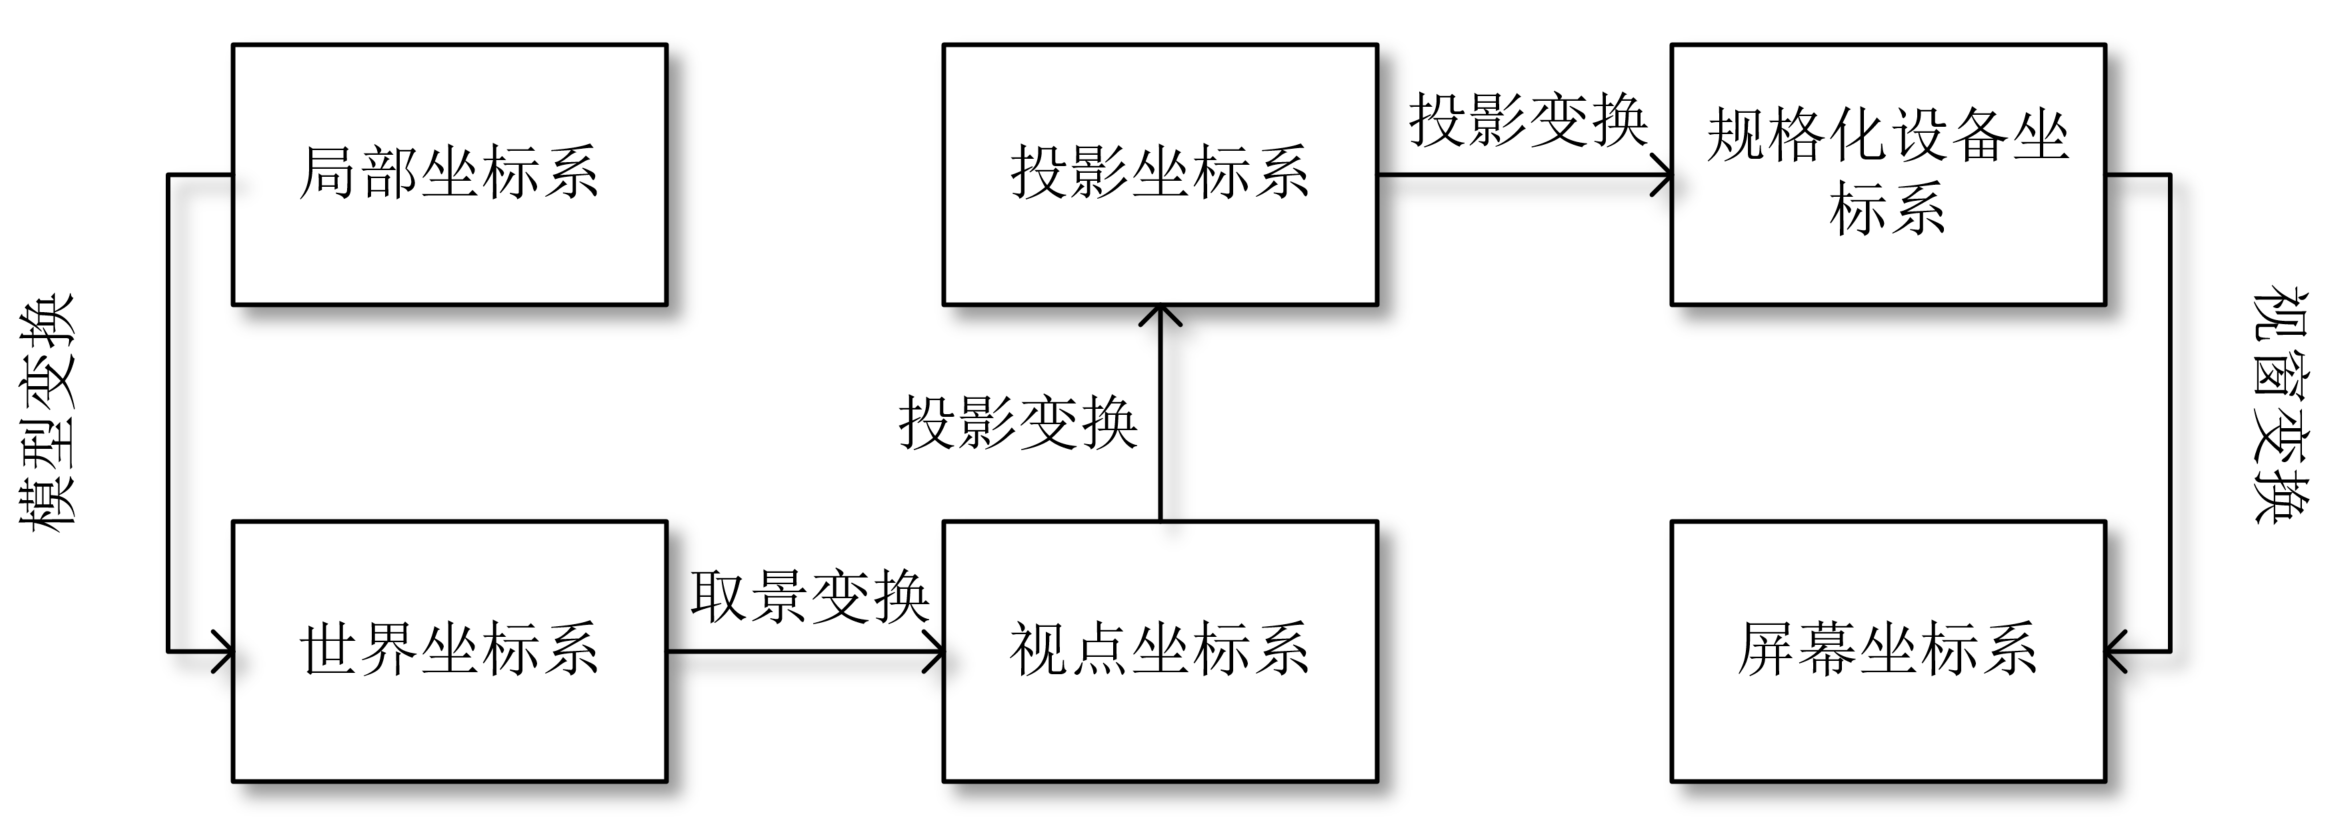
\includegraphics[scale=0.5]{coordinate.png}
\caption{常用坐标系变换}
\end{center}
\end{figure}

\subsubsection{OpenGL工程的搭建}
OpenGL是一种跨平台的图形渲染编程接口,下面总结了搭建OpenGL工程的过程。
\begin{lstlisting}
void OpenGLFunc(int argc, char** argv)
{
	glutInit(&argc, argv);
	glutInitDisplayMode(GLUT_DOUBLE | GLUT_DEPTH | GLUT_RGBA | GLUT_STENCIL);
	glutInitWindowSize(800, 600);		//set window size
	glutInitWindowPosition(100, 150);	//set window position
	glutCreateWindow("Display");		//window name
	glutDisplayFunc(DisplayFunc);		//call self defined display function
	glutIdleFunc(IdleFunc);			//call self-defined idle function
	glutKeyboardFunc(KeyboardFunc);	//call self-defined keyboard function
	glutSpecialFunc(SpecialFunc);		//call self-defined special function
	glutMouseFunc(MouseFunc);		//call self-defined mouse function
	glutMotionFunc(MotionFunc);		//call self-defined mouse motion function
	glutPassiveMotionFunc(PassiveMotionFunc);//call self-defined passive mouse motion function
	glutMainLoop();
}
\end{lstlisting}

上述代码是使得OpenGL程序能够正常运行的一个模板,该段程序为OpenGL产生的窗口设置回调函数:显示回调函数、空闲回调函数、键盘回调函数、特殊键回调函数,鼠标回调函数、鼠标按下移动回调函数和鼠标移动回调函数,他们分别定义在如下所示的函数中:
\begin{lstlisting}
	void DisplayFunc(...){...}
	void IdelFunc(...){...}
	void KeyboardFunc(...){...}
	void SpecialFunc(...){...}
	void MouseFunc(...){...}
	void MotionFunc(...){...}
	void PassiveMotionFunc(...){...}
\end{lstlisting}


\section{算法}
\subsection{数据结构}
\paragraph{活化边表}
活化边表主要存储了当前扫描线中接触到了那些边,分为两部分:(1)未画完的边;(2)顶点在该扫描线上的新加入的边。
根据$y_{max}$将边进行分类:
\begin{itemize}
\item{$x_l:$左交点的$x$坐标。}
\item{$dx_l:$左交点边上两相邻两条扫描线交点的$x$坐标差。}
\item{$dy_l:$以和左交点所在边相交的扫描线数为初值,以后向下没处理一条扫描线减一。}
\item{$x_r,dx_r,dy_r:$右边的交点的三个对应分量。}
\item{$id:$边所属多边形的编号。}
\item{$dz_x:$沿扫描线向右一个像素,多边形所在平面的深度增量。$dz_x=-\frac{a}{c}(c \neq 0)$}
\item{$dz_y:$沿$y$方向向下移动一根扫描线时,多边形所在平面的深度增量$dz_y=\frac{b}{c}(c \neq 0)$。}
\item{$id:$交点所在多边形的编号。}
\end{itemize}
\begin{figure}[H]
\setlength{\abovecaptionskip}{2pt}
\begin{center}
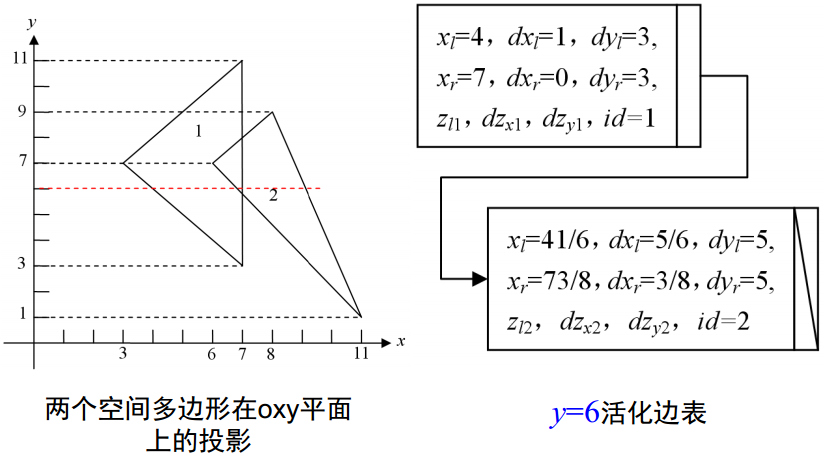
\includegraphics[scale=0.4]{structure2.png}
\end{center}
\caption{分类边表}
\end{figure}

\paragraph{活化多边形表}
根据$y_{max}$的值对多边形进行分类:
\begin{itemize}
\item{$a,b,c,d:$多边形所在平面的方程系数}
\item{$id:$多边形的编号}
\item{$dy:$多边形跨越的{\color{red} 剩余}扫描线数目}
\item{$color:$多边形的颜色}
\end{itemize}
\begin{figure}[H]
\setlength{\abovecaptionskip}{2pt}
\begin{center}
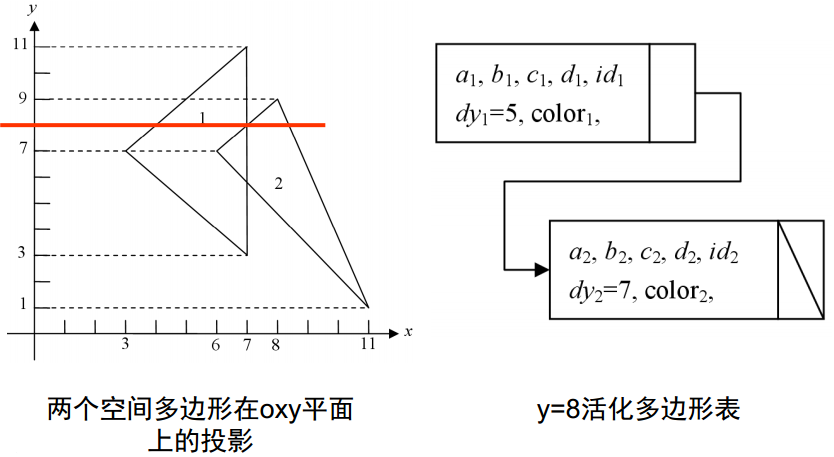
\includegraphics[scale=0.4]{structure1.png}
\end{center}
\caption{分类多边形表}
\end{figure}

\subsection{算法流程}
加载文件$\to$获取深度值$\to$消隐算法

\subsection{算法的加速}
\subsubsection{存储器的优化}

\subsubsection{取整的优化}
在扫描线算法中,需要进行大量的取整运算,c++中可以利用round函数来实现。宏相比于函数而言能够减少函数带来的开销,因此我们可以定义如下宏来代替该函数:
\begin{lstlisting}
	#define ROUND(DAT) ((int)(DAT+0.5))
\end{lstlisting}


\section{实验结果}
\subsection{实验环境}
本次实验的环境如下:
\begin{table}[H]
\caption{实验环境参数}
\begin{center}
\begin{tabular}{ll}
\toprule  %添加表格头部粗线
参数& 描述\\
\midrule  %添加表格中横线
System& Windows 10 64bit \\
CPU& Intel(R) Core(TM) i5-2410M CPU @2.30GHz 2.3GHz(4核)\\
RAM& 6GB\\
IDE& Visual Studio 2017 \\
Library& OpenGL\\
\bottomrule %添加表格底部粗线
\end{tabular}
\end{center}
\end{table}

\subsection{简单案例的设计}
在实际调试过程中会出现很多问题,为了方便调试,设计了如下所示的一些简单实例帮助调试:
\begin{figure}[H]
\setlength{\abovecaptionskip}{2pt}
\setlength{\belowcaptionskip}{20pt}
\begin{center}
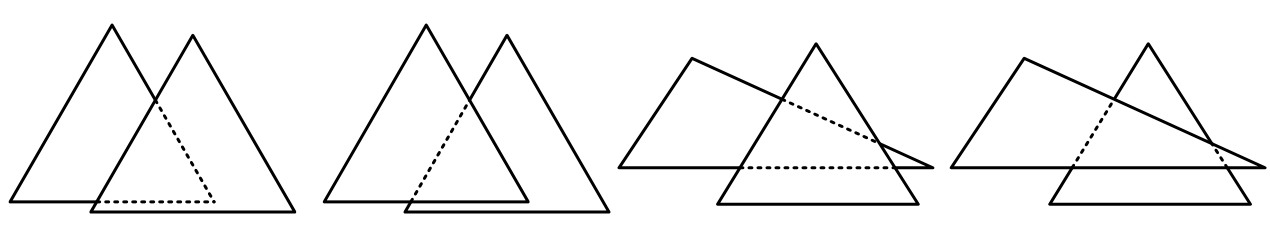
\includegraphics[scale=0.6]{cases1.png}
\caption{简单案例示意图}

\includegraphics[scale=0.5]{cases2.png}
\caption{简单案例测试效果图}
\end{center}
\end{figure}

\subsection{数据集的测试}
测试部分显示的窗口大小为$600\times600$,得到的结果如下表所示:
\begin{table}[H]
\caption{案例测试}
\begin{center}
\begin{tabular}{ccccc}
\toprule  %添加表格头部粗线
文件&三角片数&顶点数&优化前帧速(fps)\\
\midrule  %添加表格中横线
cat.obj&2755&5506&11.7883 \\
duck.obj&791&3957& 6.0306\\
bunny.obj&69451&208353&1.9299\\
\bottomrule %添加表格底部粗线
\end{tabular}
\end{center}
\end{table}

\begin{figure}[H]
\begin{center}
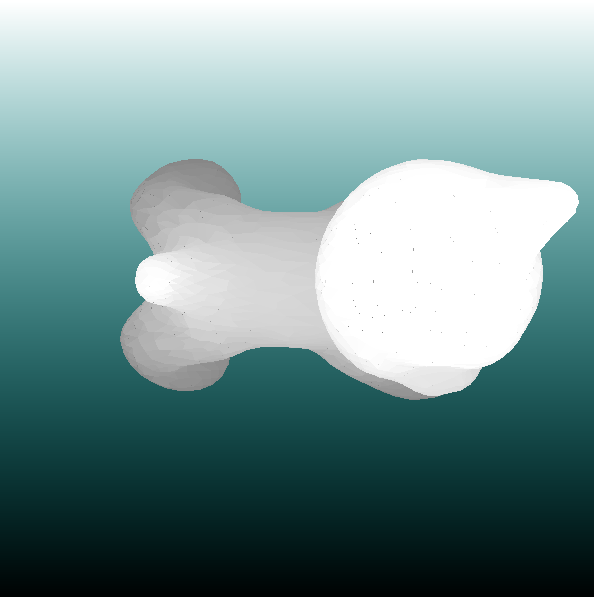
\includegraphics[scale=0.5]{cat.png}
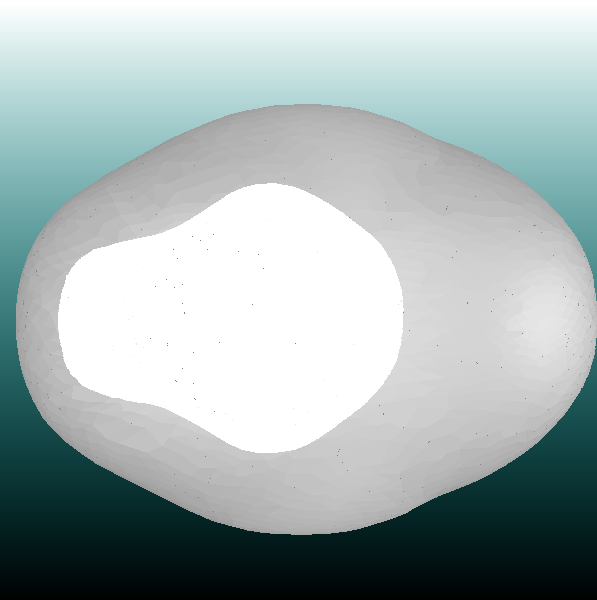
\includegraphics[scale=0.5]{duck.png}
\end{center}
\end{figure}

\begin{figure}[H]
\begin{center}
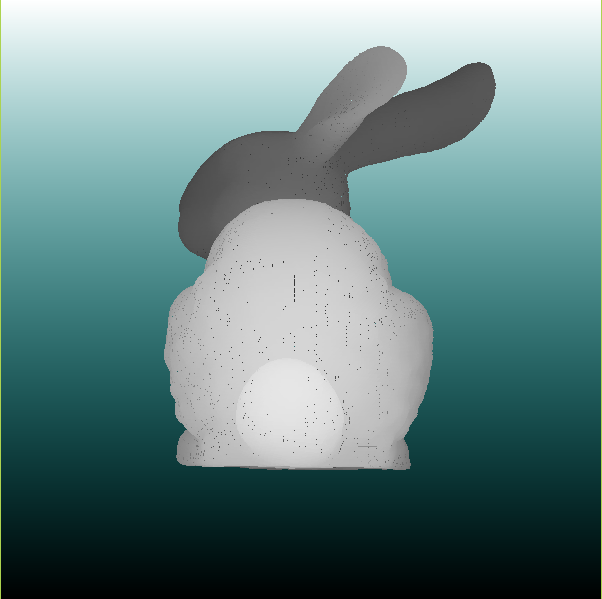
\includegraphics[scale=0.5]{bunny.png}
\end{center}
\end{figure}
\subsection{程序分析}
本次使用的是称为$bunny.obj$的文件,该文件中包含了$v$和$f$开头的数据,代码中$load\_obj.h$和$load\_obj.cpp$两个文件定义了加载$obj$文件的方法。

\section{关于一些问题的讨论}
\subsection{边状态的判定}
\paragraph{方案一:}
该方案是利用边状态的一些性质进行判断,如下所示总结出边状态的两大性质:
\begin{itemize}
\item{边的in和out状态的个数必须对应}
\item{对于扫描线扫到的同一个三角片中的边状态必定in在out之前}
\end{itemize}
\paragraph{方案二:}
如下图所示是线段$P_1P_2$为in状态的情况,假设$P_1,P_2,P_3$点对应的坐标分别为$(x_1,y_1),(x_2,y_2),(x_3,y_3)$。则线段$P_1P_2$的斜率为
\begin{equation}
k=\frac{y_1-y_2}{x_1-x_2}
\end{equation}
而线段$P_1P_2$对应的直线方程为:
\begin{equation}
\frac{y-y_1}{y_2-y_1}=\frac{x-x_1}{x_2-x_1}
\end{equation}
令
\begin{equation}
f(x,y)=\frac{y-y_1}{y_2-y_1}-\frac{x-x_1}{x_2-x_1}
\end{equation}
则当满足如下公式时则为in状态
\begin{equation}
sign(y_2-y_1)kf(x_3,y_3)<0
\end{equation}
既
\begin{equation}
(x_2-x_1)(y_3-y_1)+(y_1-y_2)(x_3-x_1)<0
\end{equation}

\begin{figure}[H]
\begin{center}
\begin{minipage}[t]{0.45\linewidth}
%\includegraphics[scale=0.7]{check_edge_status1.png}
\caption{$f(x_3,y_3)>0,k<0$}
\end{minipage}
\begin{minipage}[t]{0.45\linewidth}
%\includegraphics[scale=0.7]{check_edge_status2.png}
\caption{$f(x_3,y_3)<0,k>0$}
\end{minipage}
\end{center}
\end{figure}
\paragraph{总结:}
对比方案一和方案二不能看出方案一的思路更为简单计算量较小,因此算法中采用了方案一进行边状态的判断。
\subsection{结果中出现空白点}

\section{经验总结}
\begin{itemize}
\item{用特殊的案例对结果进行测试}
\end{itemize}

\end{document}